\chapter{Propuesta: Método de ensamble para datos desbalanceados}

%El título del capítulo es flexible de acuerdo a cada tesis. Algunos títulos sugeridos podrían ser:
%\begin{itemize}
%\item El algoritmo X: nuestra propuesta.
%\item La técnica Y
%\end{itemize}
%Este título debe de estar ade acuerdo con el asesor del tema. Consúltelo en su sala de clase.



Muchos algoritmos de clasificación han demostrado un desempeño no óptimo en problemas con clases desbalanceadas \citep{batista2004study, mani2003knn, seiffert2010rusboost}.

El ensamble es un método de aprendizaje de ensamble que podría resolver este problema si los clasificadores base fueran certeros y diversos \citep{breiman1996bagging}. Sin embargo, cada clasificador base dentro del ensamble aún sufre del mismo problema, puesto que las instancias se muestrean proporcionalmente del conjunto original. Incluso si se balancean los datos antes de ejecutar los algoritmos de aprendizaje, se altera la distribución original y se hace \textit{overfitting}.

El método de ensamble propuesto \citep{sun2015novel} ataca un problema desbalanceado convirtiéndolo en varios problemas balanceados, lo cual incluye tres componentes: \textit{Balanceo del conjunto de datos, Modelamiento y Clasificación}. La Figura \ref{fig:bagging-imbalanced} muestra los detalles.

\begin{figure}
    \centering
    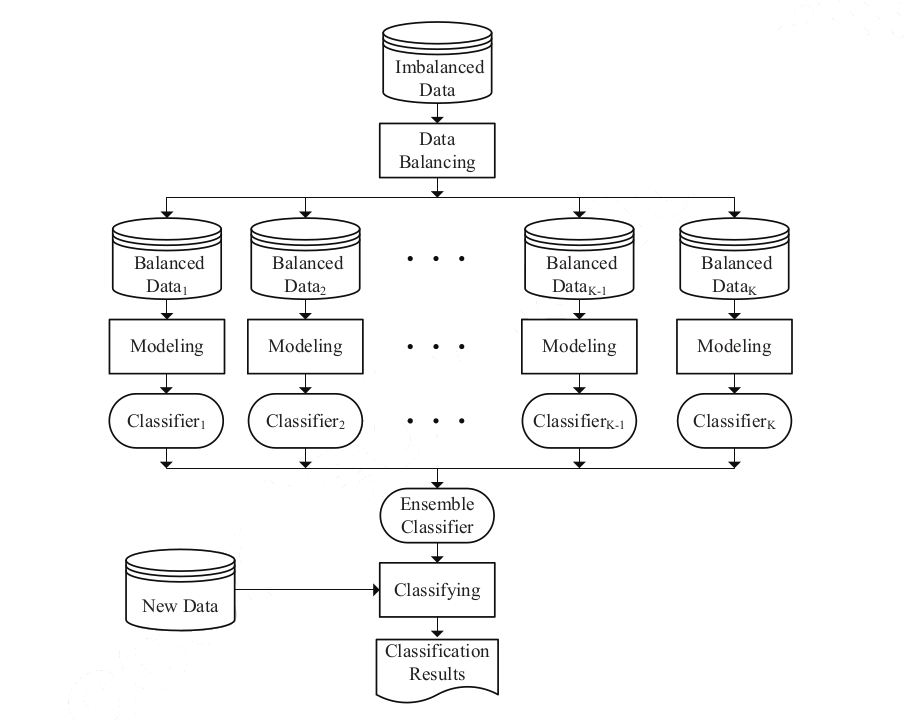
\includegraphics[width=\linewidth]{graficos/bagging_imbalanced.png}
    \caption{Método de \textit{bagging} propuesto \citep{sun2015novel}}
    \label{fig:bagging-imbalanced}
\end{figure}

En este método, la clase mayoritaria genera varios subconjuntos mediante muestreo sin repetición. Cada subconjunto tiene un número de instancias igual a la clase minoritaria, y luego se combinan con esta. Así, se obtienen varios conjuntos de datos balanceados (Balanceo de los datos). Luego, cada subconjunto se usa para crear un clasificador binario con un algoritmo específico (Modelamiento). Finalmente estos clasificadores binarios se combinan en un ensamble para clasificar nuevas instancias (Clasificación).

Esta combinación de los resultados de los clasificadores base se realiza mediante un promedio ponderado por la inversa de la distancia de la instancia a clasificar con el subconjunto utilizado. De esta manera, los subconjuntos más parecidos a la nueva instancia tendrán un mayor peso en la decisión final.

Para cumplir los objetivos de este trabajo, se implementó el algoritmo en python, usando la librería \textit{sklearn}. Se seleccionaron 3 conjuntos de datos con información creditica de diferentes características. Y se llevaron a cabo 3 experimentos para comparar el desempeño de este método con otros algoritmos del estado del arte que no se enfocan en el desbalanceo directamente. A continuación se describen los detalles al respecto.


\section{Conjuntos de datos}

Los conjuntos de datos que serán utilizados como casos de prueba son los siguientes:

\begin{description}
    \item[Apurata] Conjunto de datos privado de la \textit{fintech} peruana con el mismo nombre.
    \item[Lending Club] Conjunto de datos público de la mayor \textit{fintech} de préstamos \ac{P2P} en EE.UU \citep{dataset:lending-club}.
    \item[Crédito Alemán] Conjunto de datos público de entidades bancarias Alemanas \citep{dataset:german-credit}.
\end{description}

Una mejor comparación entre estos conjuntos se puede encontrar en la Tabla \ref{tab:dataset-comparison}

\begin{table}
    \centering
    \caption{Conjunto de datos utilizados}
    \label{tab:dataset-comparison}
    \begin{tabular}{@{}lll@{}}
    \toprule
    \textbf{Apurata}    & \textbf{Lending Club}     & \textbf{Crédito Alemán}   \\
    \midrule
    Perú (2016-2018)    & E.E.U.U (2007-2015)       & Alemania (1994)           \\
    100 - 1,000 PEN     & 1000 - 35,000 USD         & 1,000 - 20,000 EUR        \\
    1 - 9 semanas       & 36 - 60 meses             & 6 - 60 meses              \\
    626 observaciones   & 194,208 observaciones     & 1000 observaciones        \\
    33 atributos        & 46 atributos              & 24 atributos              \\
    \bottomrule
    \end{tabular}
\end{table}

Como se puede apreciar, todos los conjuntos se componen de pocas características, ninguno de ellos supera las 50. Los conjuntos de datos de Apurata y del Crédito Alemán además son pequeños respecto a la cantidad de instancias, con 1000 o menos.

También se cumple que los 3 conjuntos de datos son desbalanceados, ya que la clase de ``Moroso", representa el 15\% para Apurata, 24\% para \textit{Lending Club} y el 30\% para Crédito Alemán.

Por otro lado, los 3 conjuntos también poseen diferencias importantes entre sí que enriquecen su estudio. Apurata y \textit{Lending Club} son \textit{fintech} que utilizan diferentes criterios de los de los bancos para seleccionar su información. Los conjuntos de Crédito Alemán y \textit{Lending Club} registran créditos que se realizan por montos más altos y a un mayor plazo que los de Apurata. Los periodos de tiempo y los países abarcados por los conjuntos de datos también son únicos, y finalmente \textit{Lending Club} tiene bastante más instancias que los otros 2 conjuntos.

Hay varios estudios que utilizan el conjunto de datos Alemán \citep{harris2015credit, nanni2009experimental, brown2012experimental, wang2012two} y otros tantos que utilizan el conjunto \textit{Lending Club} \citep{malekipirbazari2015risk, zhang2016research, zang2014credit, tan2018deep}. Por lo que son considerados referenciales en sus respectivos sub-dominios.

\section{Metodología}

Para el preprocesamiento de la información, se eliminaron las variables con más del 50\% de información faltante, luego se eliminaron las filas con información faltante. A las variables resultantes se les convirtió a variables numéricas; y finalmente se hizo una normalización entre -1 y 1.

La interpretación de la variable $y$ se hizo de la siguiente manera: 1 para los buenos pagadores y 0 para los malos.

Para la selección de parámetros se realizó un \textit{grid-search} con un ajuste fino manual al final. Sobre el desbalanceo de los datos, no se tomó ningún procedimiento especial.

Para evaluar el desempeño de los modelos se hizo \textit{10-fold validation} 10 veces en Apurata y en el Crédito Alemán y 1 sola vez en \textit{Lending Club}, ya que tiene abundantes datos. Finalmente se extrajo el promedio de todas las mediciones como la medición final.

Las métricas utilizas son la exactitud, la precisión, la exhaustividad y el \ac{AUC}. La métrica que se buscó optimizar fue el \ac{AUC}. Para las otras métricas se tuvo que seleccionar un punto de corte óptimo, que se escogió tratando de optimizar la exactitud, de modo que los resultados son comparables con el estado del arte. Normalmente no se usa la exactitud para datos desbalanceados, pero ya que el estado del arte no suele tomar en cuenta el desbalanceo de las clases, la exactitud es una métrica muy utilizada en calificación crediticia, así que también se tomó en cuenta en este trabajo.


